
\chapter{Конструкторская часть}

\section{Требования к программному обеспечению}
Программа должна предоставлять следующие возможности:
\begin{enumerate}
	\item Задание положения источника света
	\item Изменения положения камеры и направления ее взгляда
	\item Визуализация трехмерных примитивов: шар, куб, цилиндр, конус
	\item Визуализация отражений, света и теней в соответствии с параметрами примитивов
	\item Поддержка перемещения и поворота заданных примитивов, а также изменения их цвета
	\item Изменения интенсивности источника света
\end{enumerate}

\section{Общий алгоритм построения изображения}
Рассмотрим алгоритм построения кадра, пока что не рассматривая конкретную реализацию алгоритма трассировки лучей на картинке~\ref{fig:frame_algo}.


\begin{figure}[H]
	\centering
	\includesvg[height=1.5\textwidth]{images/frame_algo}
	\caption{Общий алгоритм построения кадра}
	\label{fig:frame_algo}
\end{figure}



\section{Выбор типов и структур данных}
В данной работе необходимо создание следующих структур данных:
\begin{enumerate}
	\item Структура точки описывается следующими полями
	\begin{enumerate}[label*=\arabic*.]
		\item X - координата точки по оси X.
		\item Y - координата точки по оси Y.
		\item Z - координата точки по оси Z.
	\end{enumerate}

	\item Структура трехмерного вектора описывается следующими полями:
	\begin{enumerate}[label*=\arabic*.]
		\item X - Направление вектора по  оси X.
		\item Y - Направление вектора  по оси Y.
		\item Z - Направление вектора  по оси Z.
	\end{enumerate}

	\item Структура цвета описывается следующими полями:
	\begin{enumerate}[label*=\arabic*.]
		\item R - интенсивность красного цвета.
		\item G - интенсивность зеленого цвета.
		\item B - интенсивность синего цвета.
	\end{enumerate}

	\item Структура источника света описывается следующими полями:
	\begin{enumerate}[label*=\arabic*.]
		\item Position - вектор положения источника света в пространстве.
		\item Color - интенсивность источника света по каждой составляющей RGB.
	\end{enumerate}

	\item Структура камеры описывается следующими полями:
	\begin{enumerate}[label*=\arabic*.]
		\item Position - вектор положения камеры в пространстве.
		\item Direction - вектор направления взгляда камеры.
		\item 2 вектора, которые вместе с Direction задают систему координат камеры: Up, Right.
	\end{enumerate}
	
	\item Структура материала объекта описывается следующими полями:
	\begin{enumerate}[label*=\arabic*.]
		\item Color - цвет данного материала.
		\item kA - коэффициент рассеянного освещения.
		\item kD - коэффициент диффузного освещения.
		\item kS - коэффициент спектрального освещения.
	\end{enumerate}


	\item Структура луча описывается следующими полями:
	\begin{enumerate}[label*=\arabic*.]
		\item Position - точка, лежащая на данном луче.
		\item Direction - вектор задающий направление луча.
		\item t - вещественное число, задающее точку на данном луче.
	\end{enumerate}

	\item Сцена содержит массив трехмерных примитивов
	\item Примитивы задаются аналогично их формальному описанию (см.\ref{sec:obj_formalasation})
\end{enumerate}



\section{Алгоритм обратной трассировки лучей}
Алгоритм трассировки лучей для 1 пикселя приведен на картинке~\ref{fig:raytrace_algo_pixel}. Входными данными для него являются: описания объектов, число пикселей на экране,
интенсивность источника света.

\begin{figure}[H]
	\centering
	\includesvg[height=1.5\textwidth]{images/raytrace_pixel}
	\caption{Алгоритм трассировки лучей для 1 пикселя}
	\label{fig:raytrace_algo_pixel}
\end{figure}

Теоретически свет может отражаться бесконечно, введение ограничения на максимальное число поколений луча позволит ограничить время построения изображения.
Необходимо отметить, что каждый луч при пересечении с поверхностью образует 2 луча: преломленный и отраженный, таким образом можно построить дерево расчета лучей.
Пример такого дерева приведен на картинке~\ref{fig:raytrace_tree}, на данном дереве левая ветвь соответствует лучам, полученным в результате отражения, правая - в результате преломления,
стрелками указан обход дерева, при спуске по дереву луч строится, при поднятии по дереву интенсивность вычисляется. Можно заметить что максимальное поколение лучей является максимальной высотой получаемого дерева.

В данном случае при помещении луча в стек кладутся его следующие параметры:
\begin{enumerate}
	\item Вычисленная интенсивность 
	\item Параметры луча для составления его уравнения 
	\item Текущее поколение \cite{Rodgers}
\end{enumerate}



\begin{figure}[h]
	\centering
	\includesvg[scale=0.8]{images/raytrace_tree}
	\caption{Пример дерева трассировки луча}
	\label{fig:raytrace_tree}
\end{figure}

\subsection{Расчет интенсивности света в соответствии с выбранной моделью}
На картинке~\ref{fig:raytrace_algo_pixel} необходимо рассчитать интенсивность света, рассмотрим как это будет происходить в соответствии с моделью освещения Уиттеда. (см~\ref{fig:global_reflections})
\begin{figure}[H]
	\centering
	\includesvg[height=1.3\textwidth,width=1\textwidth]{images/Yuitted_model}
	\caption{Алгоритм вычисления интенсивности света для модели Уиттеда}
	\label{fig:yuitted_model_algo}
\end{figure}
Если изображение цветное то приведенный блок (см.~\ref{fig:yuitted_model_algo}) выполняется трижды - для каждого из основных цветов. Идея данного алгоритма проста:
в случае если вектор от источника света к рассматриваемой точке пересекает непрозрачное тело, источник света не освещает данную точку и мы переходим к следующему,
если существует пересечение с прозрачными объектами, то они поглотят часть света и его интенсивность снизится. Заметим, что в данной реализации преломление света в прозрачных телах не учитывается.
Считается, что нормаль к поверхности в заданной точке можно получить из описания объекта. (см.~\ref{sec:obj_formalasation}).
Рисунок~\ref{fig:yuitted_model_algo} соответствует этапу <<Вычислить интенсивность света \(I\) в данной точке>> в алгоритме обратной трассировки лучей (см.~\ref{fig:raytrace_algo_pixel}).
Данная модель освещения может быть модифицирована для учета преломления света. \cite{Rodgers}

\subsection{Нахождение пересечения с объектами сцены}
Один из самых трудозатратных этапов данного алгоритма  - поиск пересечения с объектами сцены. Необходимо быстро определять координаты точки пересечения испущенного луча 
с данными примитивами.


Для начала необходимо ввести уравнение самого луча (см.~\ref{eq:ray_vector_eq}).
\begin{equation} 
	P(t) = \vec{E} +t\vec{D},t \ge 0
	\label{eq:ray_vector_eq}
\end{equation}
Также уравнение~\ref{eq:ray_vector_eq} имеет запись
\begin{equation}
	\label{eq:ray_scalar_eq}
	\begin{aligned}
		x(t) = x_E + t x_D \\
		y(t) = y_E + t y_D \\
		z(t) = z_E + t z_D.
	\end{aligned}
\end{equation}
Таким образом луч определяется: точкой обзора - $\vec{E} = (x_E,y_E,z_E)$ и вектором направления - $\vec{D} = (x_D,y_D,z_D)$. Значение $t$  определяет направление луча: в случае если $t ge 0$,
точка на луче находится после точки обзора, иначе - за. Таким образом для поиска наиближайшей точки пересечения, необходимо найти наименьшее неотрицательное значение $t$.\cite{Rodgers,primitives_raytracing_equations} 


\textbf{Уравнение сферы}
Сфера с единичным радиусом может быть задана следующим образом:
\begin{equation}
	\vec{P} \cdot \vec{P}=1
	\label{eq:sphere_eq}
\end{equation}
Для получения условия пересечений достаточно подставить уравнение луча из~\ref{eq:ray_vector_eq} в~\ref{eq:sphere_eq} и решить полученное уравнение относительно t.
\begin{equation}
	t=\frac{-b\pm\sqrt{b^2-4ac}}{2a}
	\label{eq:sphere_solved}
\end{equation}
После проведенных преобразований будет получена формула~\ref{eq:sphere_solved}, где:
\begin{enumerate}
	\item $a = \vec{D} \cdot \vec{D}$ 
	\item $b = 2\vec{E} \cdot \vec{D}$ 
	\item $c = \vec{E} \cdot \vec{E} - 1$
\end{enumerate}
В случае если вещественные решения уравнения~\ref{eq:sphere_solved} отсутствуют, то пересечения луча также отсутствуют, если только одно решение  - существует одно
пересечение и т.~д. Если значение отрицательное то точка пересечения находится за точкой наблюдения и нас не интересует.\cite{primitives_raytracing_equations}

\textbf{Уравнение цилиндра}
Уравнение~\ref{eq:cylinder_eq} задает бесконечный цилиндр.
\begin{equation}
	x^2 + y^2=1
	\label{eq:cylinder_eq}
\end{equation}
Для ограничения цилиндра необходимо ввести требования к значению $z$ цилиндра:
\begin{equation}
	x^2 + y^2=1,z_{\min} < z  < z_{\max}	
	\label{eq:cylinder_eq_demanding}
\end{equation}
Для нахождения пересечений подставим~\ref{eq:ray_scalar_eq} в~\ref{eq:cylinder_eq}, после чего получим уравнение~\ref{eq:inf_cylinder_solved}
\begin{equation}
	t=\frac{-b\pm\sqrt{b^2-4ac}}{2a}
	\label{eq:inf_cylinder_solved}
\end{equation}
В формуле~\ref{eq:inf_cylinder_solved}:
\begin{enumerate}
	\item $a = x_{D}^2 + y_{D}^2$ 
	\item $b = 2x_Ex_D+2y_Ey_D$ 
	\item $c = x_{E}^2+y_{E}^2 - 1$
\end{enumerate}

После вычисления значения по данной формуле, будет получено  одно или несколько значений $t$, для конечного цилиндра необходимо вычислить значения $z$ по
формуле~\ref{eq:ray_scalar_eq} ($z_1 = z_E + t_1z_D,z_2 = z_E + t_2z_D$), после чего проверить соответствуют ли полученные значения $z$ условию $z_{\min} < z  < z_{\max}$.
Также необходимо проверить пересечения луча с верхней и нижней окружностями цилиндра, для этого можно воспользоваться формулами:
\begin{equation}
	\label{eq:cylinder_caps}
	\begin{aligned}
		x^2 + y^2=1,z = z_{\min}\\
		x^2 + y^2=1,z = z_{\max}.
	\end{aligned}
\end{equation}
Если $z_1,z_2$ лежат с разных сторон от $z_{\min}$, то луч проходит через ближайшую окружность цилиндра и вычислить значение $t$ можно следующим способом:
\begin{equation}
	t_3=\frac{z_{\min}-z_E}{z_D}.
	\label{eq:cylinder_caps_solved}
\end{equation}
Аналогично находится и точка пересечения с дальней окружностью ($z_{\max}$) цилиндра.\cite{primitives_raytracing_equations}


\textbf{Уравнение конуса}
Конус задается уравнением~\ref{eq:cone_eq}
\begin{equation}
	x^2+y^2=z^2.
	\label{eq:cone_eq}
\end{equation}
После введения данного уравнения точка пересечения вычисляется аналогично точке пересечения с цилиндром. Нельзя забывать, что так же как и в работе с цилиндром, для
ограничения фигуры необходимо вводить условия $z_{\min} < z < z_{\max}$.

\textbf{Уравнение плоскости}
Плоскость может определяться вектором нормали $\vec{N}$, и вершиной на плоскости $Q$. Таким образом точка $P$ принадлежит плоскости, если 
\begin{equation}
	\vec{N} \cdot (\vec{P} - \vec{Q}) = 0.
	\label{eq:plane_eq}
\end{equation}

Для нахождения пересечения необходимо подставить~\ref{eq:ray_vector_eq} в~\ref{eq:plane_eq}. После выполнения преобразований будет получено
выражение~\ref{eq:plane_eq_solved}.
\begin{equation}
	t=\frac{\vec{N} \cdot (\vec{Q} - \vec{E})}{\vec{N} \cdot \vec{D}}
	\label{eq:plane_eq_solved}
\end{equation}
В случае, если $t \ge 0$ тогда точка пересечения $\vec{E} + t\vec{D}$. Если $\vec{N} \cdot \vec{D} = 0$ тогда луч параллелен плоскости и
точка пересечения отсутствует.\cite{primitives_raytracing_equations}


\textbf{Трансформация примитивов}
Заметим что в записанных нами формулах наложены ограничения на положение фигур:
\begin{enumerate}
	\item Сфера и цилиндр были рассмотрены только с единичным радиусом
	\item Цилиндр и конус совмещены по оси с осью $z$
	\item Конус имеет единичный уклон
\end{enumerate}
Для поиска пересечения необходимо найти преобразования, переводящие примитив из начала координат и данных условий в требуемые (перенос, поворот, масштабирование).
После чего применить обратные преобразования к построенному лучу.
Пусть объект $\hat{B}$ проходит трансформацию $TRS$, чтобы попасть в требуемую позицию $B = TRS\hat{B}$, в таком случае обратное преобразование луча будет выглядеть
следующим образом (см.~\ref{eq:primitives_transformation}).
\begin{equation}
	\label{eq:primitives_transformation}
	\begin{aligned}
		\hat{E} = S^{-1}R^{-1}T^{-1}\vec{E}\\
		\hat{D} = S^{-1}R^{-1}\vec{D}.
	\end{aligned}
\end{equation}
После нахождения пересечения преобразованного луча с исходным объектом будет получено значение $t$, что позволяет посчитать $\vec{P} = \vec{E} +t\vec{D}$.

\section{Перспектива}
Для получения перспективы необходимо cкорректировать направление каждого луча. Перед тем как получить наше изображение необходимо спроецировать его на картинную плоскость.
%TODO: описать что такое картинная плоскость и найти картинку получше
все лучи должны исходить из одной точки и проходить через полученные соответствующие пиксели (см.~\ref{fig:perspective_view}).Для описания координатной системы камеры введены:
вектора $-w$ - вектор направления взгляда, $\mathrm{e}$ - точка наблюдения, $\mathrm{v}$ - вектор направленный <<вверх>> (англ. up vector), необходимый для построения базиса.
В данном случае картинная плоскость находится на удалении $d$ в направлении взгляда $\mathrm{-w}$, каждый луч будет иметь различное направление в зависимости от пересекаемого пикселя.
\begin{figure}[H]
	\centering
	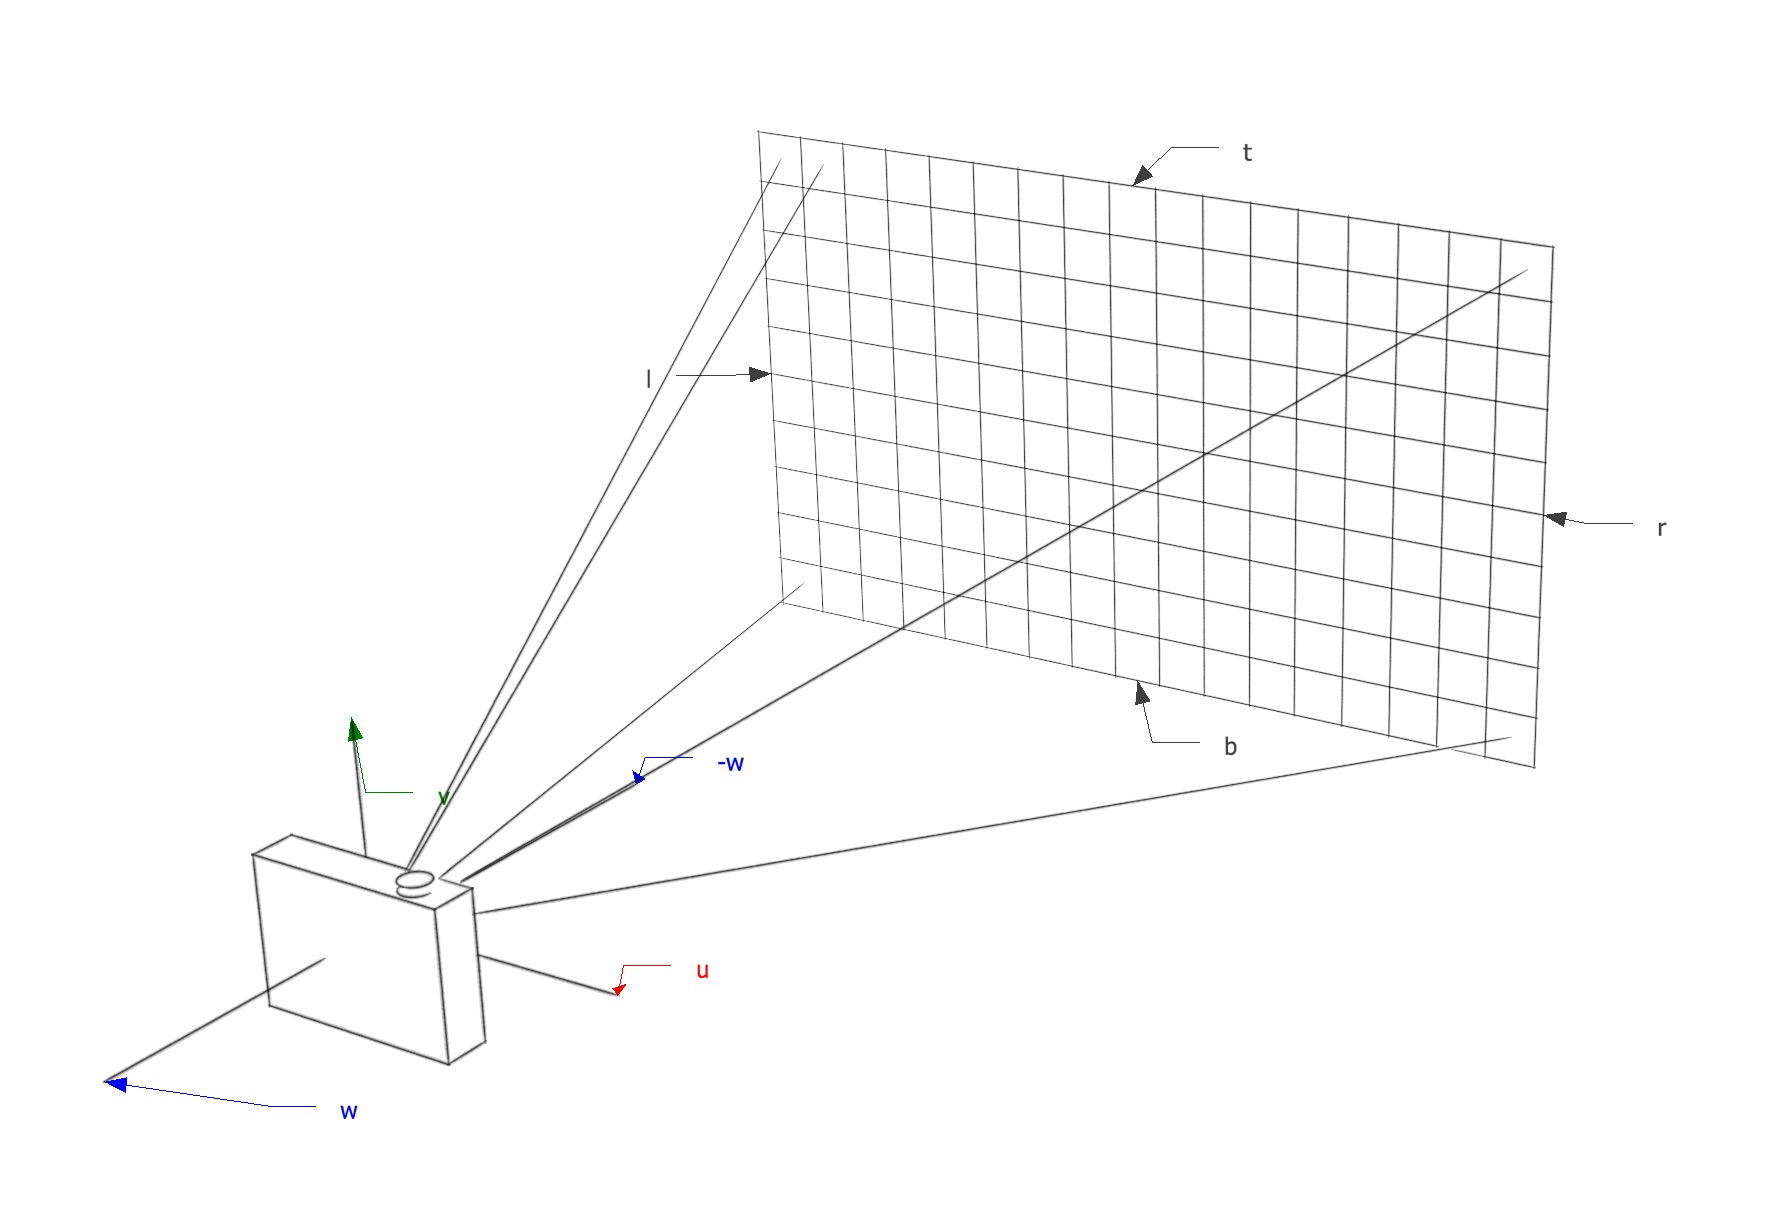
\includegraphics[scale=0.3]{raytracing_perspective}
	\caption{Перспективный вид}
	\label{fig:perspective_view}
\end{figure}
Соответственно необходимо корректировать вектор направления испускаемых лучей (см.~\ref{eq:ray_vector_eq}) следующим образом:
\begin{equation}
	D = -d\mathrm{w} + u\mathrm{n} + u\mathrm{v}
\end{equation}
где $u,v$ получены из расчета луча для каждого пикселя (см.~\ref{eq:pixel_rays}).
\begin{equation}
	\begin{aligned}
		u = l + (x + 0.5)\frac{r - l}{n_x}\\
		v = b + (y + 0.5)\frac{t - b}{n_y}.
	\end{aligned}
	\label{eq:pixel_rays}
\end{equation}
В выражениях~\ref{eq:pixel_rays} символы соответственно означают:
\begin{enumerate}
	\item $l,r$ - Позиции левого  и правого краев изображения соответственно
	\item $t,b$ - Позиции верхнего и нижнего краев изображения соответственно
	\item $x,y$ - Координаты пикселя
	\item $n_x,n_y$ - Количество пикселей по соответствующим осям изображения
\end{enumerate}

После выполненных преобразований будет получено представления луча, для которого будут вычисляться
пересечения с объектами.\cite{perspective_raytracing}



\textbf{Выводы}

В данном разделе была разобрана реализация выбранного алгоритма построения изображения, а также рассмотрены случаи поиска пересечений лучей  к конкретным примитивам. 
Была затронута тема построения перспективы для выбранного алгоритма и математическое обоснование его работы. Были описаны основные структуры данных, необходимы для решения поставленных задач.




